\documentclass{beamer}
\usetheme{default}
\setbeamertemplate{navigation symbols}{}
\usepackage{amsmath,amssymb,booktabs,multirow}
\usepackage{listings,xcolor}
\usepackage{tikz}
\usetikzlibrary{positioning,arrows.meta,shapes}
\usepackage{algorithm,algpseudocode}
\graphicspath{{img/}}
\lstset{basicstyle=\ttfamily\small,keywordstyle=\color{blue}\bfseries,commentstyle=\color{gray},
  stringstyle=\color{red!60!black},language=Python,columns=fullflexible}

\begin{document}

\begin{frame}{Two text columns}
  \begin{columns}[T]
    \column{0.48\textwidth}
    \textbf{Before}
    \begin{itemize}
      \item Manual copy-paste
      \item Lost formatting
      \item Hours per talk
    \end{itemize}
    \column{0.48\textwidth}
    \textbf{After}
    \begin{itemize}
      \item One command
      \item Same layout
      \item Minutes per talk
    \end{itemize}
  \end{columns}
  \vfill
  \centering\small Footer remark in the middle of the frame.
\end{frame}

\begin{frame}[fragile]{Highlighted code}
\begin{lstlisting}
def convert(pdf):
    # classify every page
    for page in pages(pdf):
        emit(page, "slides")
\end{lstlisting}
  Code with keywords, comments and strings.
\end{frame}

\begin{frame}{A table with rules and merged cells}
  \centering
  \begin{tabular}{|l|c|c|}
    \hline
    \multirow{2}{*}{Model} & \multicolumn{2}{c|}{Score} \\
    \cline{2-3}
     & Train & Test \\
    \hline
    Linear & 0.80 & 0.78 \\
    Tree & 0.95 & 0.81 \\
    \hline
  \end{tabular}
\end{frame}

\begin{frame}{Algorithm}
  \begin{algorithmic}[1]
    \Require a PDF deck $D$
    \For{each page $p$ in $D$}
      \State classify $p$
      \If{$p$ has text}
        \State emit text boxes
      \EndIf
    \EndFor
  \end{algorithmic}
\end{frame}

\begin{frame}{Diagram with circles and edge labels}
  \centering
  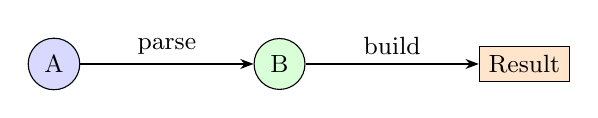
\begin{tikzpicture}[node distance=2.2cm, every node/.style={font=\small}]
    \node[circle, draw, fill=blue!15] (a) {A};
    \node[circle, draw, fill=green!15, right=of a] (b) {B};
    \node[draw, fill=orange!20, right=of b] (c) {Result};
    \draw[-{Stealth}] (a) -- node[above] {parse} (b);
    \draw[-{Stealth}] (b) -- node[above] {build} (c);
  \end{tikzpicture}

  \vspace{1em}
  \begin{itemize}
    \item Circles, rectangles and labelled edges
  \end{itemize}
\end{frame}

\begin{frame}{Footnotes and colored words}
  \begin{itemize}
    \item Some \textcolor{red}{red} and \textcolor{blue}{blue} words
    \item A claim that needs a source\footnote{Author et al., 2024.}
    \item \colorbox{yellow}{Highlighted} text and \underline{underlined} text
    \item \small smaller \normalsize and \large larger \normalsize text
  \end{itemize}
\end{frame}

\end{document}
